% Paquets généraux
\documentclass[a4paper,12pt,titlepage]{article}
\usepackage[T1]{fontenc}
\usepackage[utf8]{inputenc}
\usepackage[french]{babel}
\usepackage[gen]{eurosym}
%\usepackage[dvips]{graphicx}
\usepackage{fancyhdr}
\usepackage{pdfpages} 
\usepackage{multido}
\usepackage{hyperref}
%\usepackage{textcomp}
%\usepackage{aeguill}
\usepackage{schemabloc}
\usepackage[bitstream-charter]{mathdesign}
\usepackage{pstricks}
\usepackage{helvet}

\newcommand{\id}{54}
\newcommand{\nom}{Liaisons mécaniques}
\newcommand{\sequence}{04}
\newcommand{\num}{01}
\newcommand{\type}{TP}
\newcommand{\descrip}{Modélisation d'un solide. Comportement des liaisons mécaniques. Modéliser les mécanismes du laboratoire par un schéma cinématique, paramétré.}
\newcommand{\competences}{A3-C4: Analyse d'architecture et de comportement \\ &  Mod1-C1: Isolement d'un solide ou d'un système de solides \\ &  Mod2-C10-1: Modèle de solide indéformable \\ &  Mod2-C11: Modélisation géométrique et cinématique des mouvements entre solides indéformables \\ &  Mod2-C12: Modélisation cinématique des liaisons entre solides \\ &  Mod2-C15: Modélisation des actions mécaniques \\ &  Rés-C6: Utilisation d'un solveur ou d'un logiciel multi physique \\ &  Com1-C1: Différents descripteurs introduits dans le programme \\ &  Com2-C4: Outils de communication}
\newcommand{\nbcomp}{9}
\newcommand{\systemes}{Plateforme Stewart}
\newcommand{\systemessansaccent}{Plateforme Stewart}
\newcommand{\ilot}{2}
\newcommand{\ilotstr}{02}
\newcommand{\dossierilot}{\detokenize{Ilot_02 Plateforme Stewart}}
\newcommand{\imageun}{Plateforme}

\newcommand{\urlsysteme}{\href{https://www.costadoat.fr/systeme/57}{Ressources système}}
\newcommand{\matlabsimscape}{\href{https://github.com/Costadoat/Sciences-Ingenieur/raw/master/Systemes/Plateforme Stewart/Plateforme_Stewart_Simscape.zip}{Modèle Simscape}}
\newcommand{\solidworks}{\href{https://github.com/Costadoat/Sciences-Ingenieur/raw/master/Systemes/Plateforme Stewart/Plateforme_Stewart_Solidworks.zip}{Modèle Solidworks}}
\newcommand{\edrawings}{\href{https://github.com/Costadoat/Sciences-Ingenieur/raw/master/Systemes/Plateforme Stewart/Plateforme_Stewart.EASM}{Modèle eDrawings}}
\newcommand{\test}{Stewart_param1}
\newcommand{\testi}{Stewart_param2}
\newcommand{\testii}{Stewart_param3}
\newcommand{\testiii}{Stewart_param4}
\newcommand{\testiiii}{Stewart_euler}

\newcommand{\auteurun}{Renaud Costadoat}
\newcommand{\institute}{Lycée Dorian}


\usepackage{color}
\usepackage{xcolor}
\usepackage{colortbl}
\usepackage{helvet}
\renewcommand{\familydefault}{\sfdefault}
\usepackage{amsfonts}
\usepackage{amsmath}
%\usepackage{xspace}
\usepackage{varioref}
\usepackage{tabularx}
%\usepackage{floatflt}
\usepackage{graphics}
\usepackage{wrapfig}
\usepackage{textcomp}
\usepackage{tikz}
\usepackage{wrapfig}
\usepackage{gensymb}
\usepackage[european]{circuitikz}
\usetikzlibrary{babel}
\usepackage{ifthen}
\usepackage{cancel}
\usepackage{etoolbox}
\usepackage{multirow}
%\usepackage{boxedminipage}
\definecolor{gris25}{gray}{0.75}
\definecolor{bleu}{RGB}{18,33,98}
\definecolor{bleuf}{RGB}{42,94,171}
\definecolor{bleuc}{RGB}{231,239,247}
\definecolor{rougef}{RGB}{185,18,27}
\definecolor{rougec}{RGB}{255,188,204}%255,230,231
\definecolor{vertf}{RGB}{103,126,82}
\definecolor{vertc}{RGB}{220,255,191}
\definecolor{forestgreen}{rgb}{0.13,0.54,0.13}
\definecolor{blcr}{rgb}{0.59,0.69,0.84}
\definecolor{blfr}{rgb}{0.32,0.51,0.75}
\definecolor{orfr}{rgb}{0.90,0.42,0.15}
\definecolor{orcr}{rgb}{0.90,0.65,0.50}
\definecolor{orangef}{rgb}{0.659,0.269,0.072}
\definecolor{orange}{rgb}{0.58,0.35,0.063}
\definecolor{orangec}{rgb}{0.43,0.32,0.25}
\definecolor{rcorrect}{rgb}{0.6,0,0}
\definecolor{sequence}{rgb}{0.75,0.75,0.75}
\definecolor{competences}{rgb}{0.61,0.73,0.35}
\definecolor{grisf}{HTML}{222222}
\definecolor{grisc}{HTML}{636363}
\definecolor{normal}{HTML}{4087c4}
\definecolor{info}{HTML}{5bc0de}
\definecolor{success}{RGB}{92,184,92}
\definecolor{warning}{RGB}{240,173,78}
\definecolor{danger}{RGB}{217,83,79}
\hypersetup{                    % parametrage des hyperliens
    colorlinks=true,                % colorise les liens
    breaklinks=true,                % permet les retours à la ligne pour les liens trop longs
    urlcolor= blfr,                 % couleur des hyperliens
    linkcolor= orange,                % couleur des liens internes aux documents (index, figures, tableaux, equations,...)
    citecolor= forestgreen                % couleur des liens vers les references bibliographiques
    }

% Mise en page
\pagestyle{fancy}

\setlength{\hoffset}{-18pt}

\setlength{\oddsidemargin}{0pt} 	% Marge gauche sur pages impaire2s
\setlength{\evensidemargin}{0pt} 	% Marge gauche sur pages paires
\setlength{\marginparwidth}{00pt} 	% Largeur de note dans la marge
\setlength{\headwidth}{481pt} 	 	% Largeur de la zone de tête (17cm)
\setlength{\textwidth}{481pt} 	 	% Largeu\textbf{r de la zone de texte (17cm)
\setlength{\voffset}{-18pt} 		% Bon pour DOS
\setlength{\marginparsep}{7pt}	 	% Séparation de la marge
\setlength{\topmargin}{-30pt} 		% Pas de marge en haut
\setlength{\headheight}{55pt} 		% Haut de page
\setlength{\headsep}{20pt} 		% Entre le haut de page et le texte
\setlength{\footskip}{30pt} 		% Bas de\textbf{ page + séparation
\setlength{\textheight}{700pt} 		% Hauteur de l'icone zone de texte (25cm)
\setlength\fboxrule{1 pt}
\renewcommand{\baselinestretch}{1}
\setcounter{tocdepth}{1}
\newcommand{\cadre}[2]
{\fbox{
  \begin{minipage}{#1\linewidth}
   \begin{center}
    #2\\
   \end{center}
  \end{minipage}
 }
}

\newcommand{\reponse}[1][4]
{
\multido{}{#1}
{\begin{center}\makebox[0.9\linewidth]{}  \\
\begin{center}\makebox[0.9\linewidth]{\dotfill} \\ \end{center}
}}

\newcommand{\titre}[1]
{\begin{center}
\cadre{0.8}{\huge #1} 
\end{center}
}


% En tête et pied de page
\lhead{\nom}
\rhead{
\includegraphics[width=2cm]{../../img/logo}}
\lfoot{Renaud Costadoat}
\cfoot{Page \thepage}

\fancypagestyle{correction}{%
  \fancyhf{}
  \lhead{\colorbox{danger}{\begin{minipage}{0.65\paperwidth} \textcolor{white}{\textbf{Correction}} \end{minipage}} }
  \rhead{
\includegraphics[width=2cm]{../../img/logo}}
  \lfoot{Renaud Costadoat}
  \rfoot{\colorbox{danger}{\begin{minipage}{0.6\paperwidth} \begin{flushright}\textcolor{white}{\textbf{Correction}}\end{flushright} \end{minipage}} }}

\renewcommand{\footrulewidth}{0.4pt}

\usepackage{eso-pic}
\newcommand{\BackgroundPic}{%
\put(0,0){%
\parbox[b][\paperheight]{\paperwidth}{%
\vfill
\begin{center}
\hspace{0.5cm}\vspace{0.5cm}
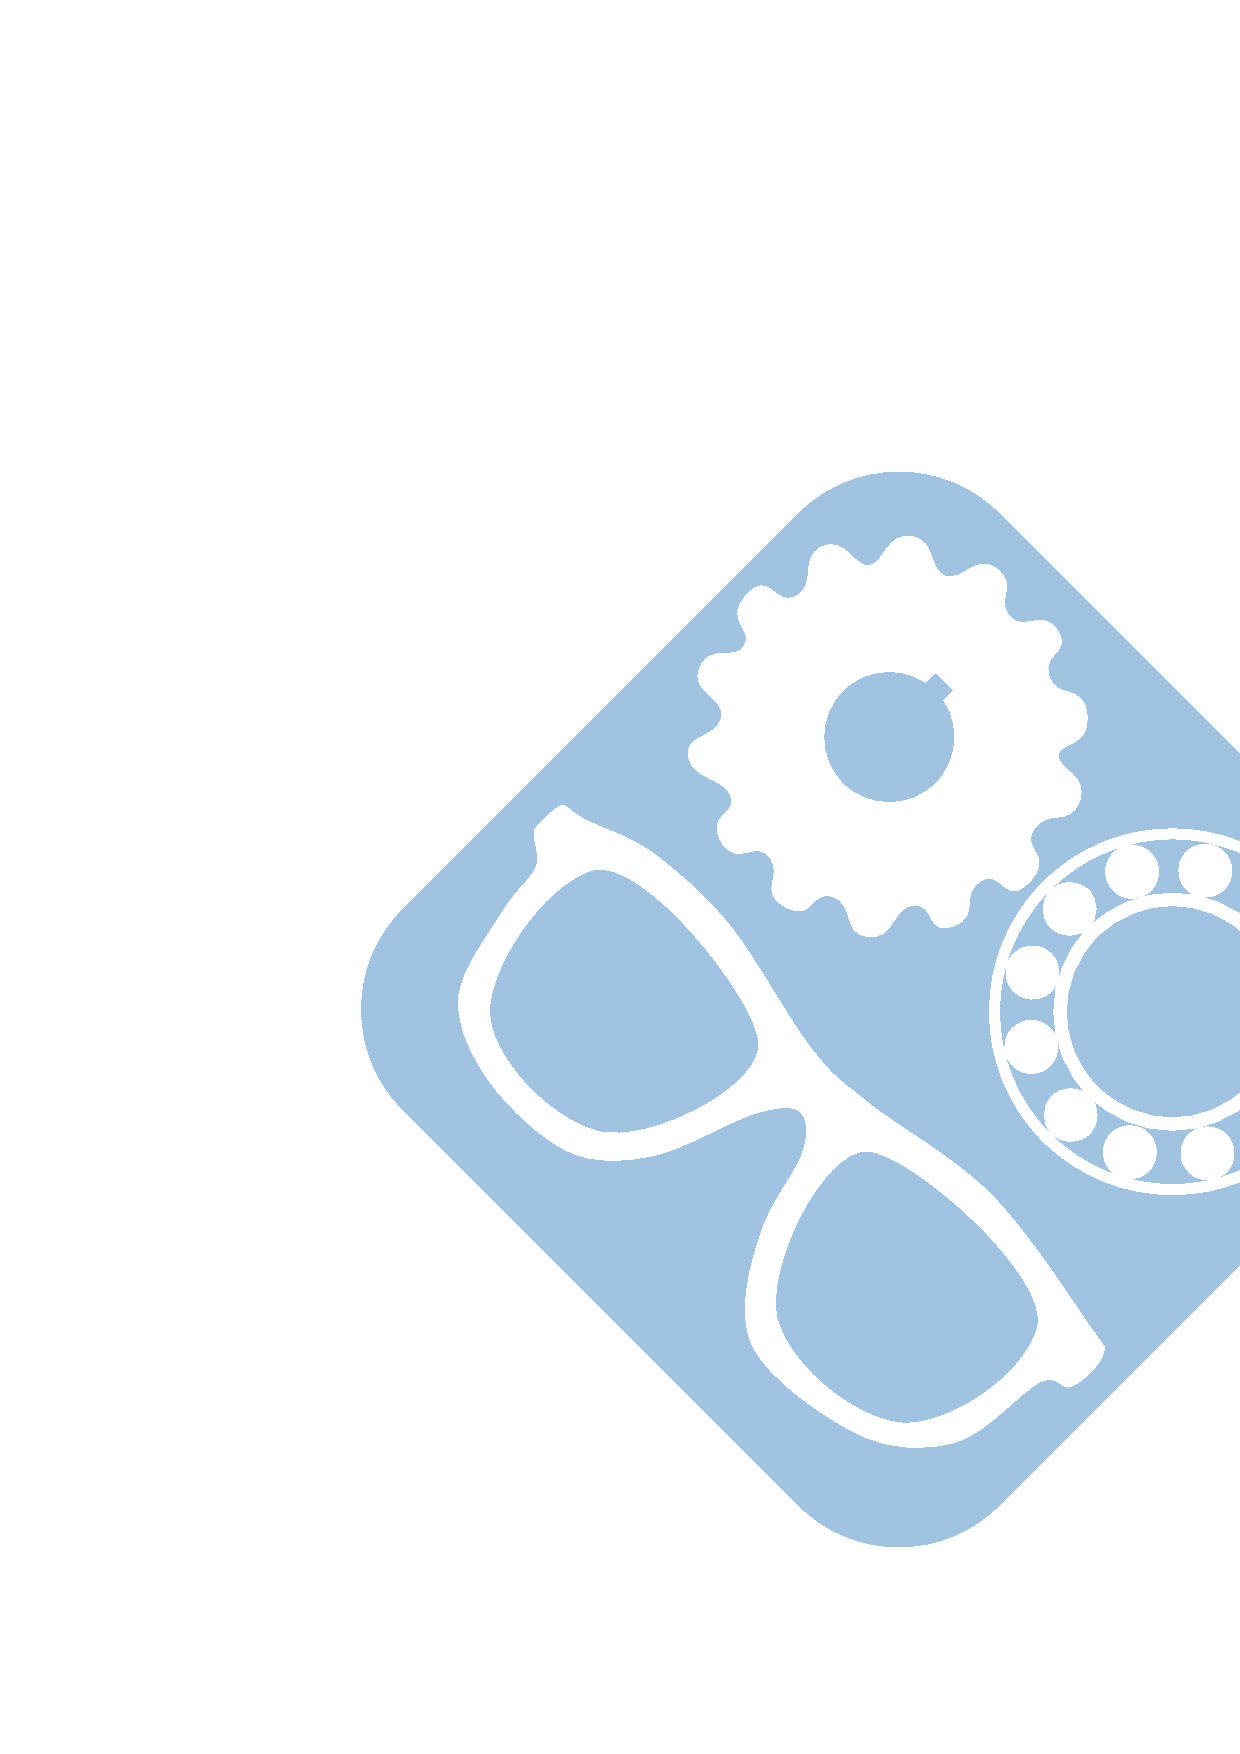
\includegraphics[width=\paperwidth,height=\paperheight,%
keepaspectratio]{../../img/fond3}%
\end{center}
\vfill
}}}

\newcommand{\BackgroundPicdeux}{%
\put(25,-30){%
\parbox[b][\paperheight]{\paperwidth}{%
\vfill
\begin{center}
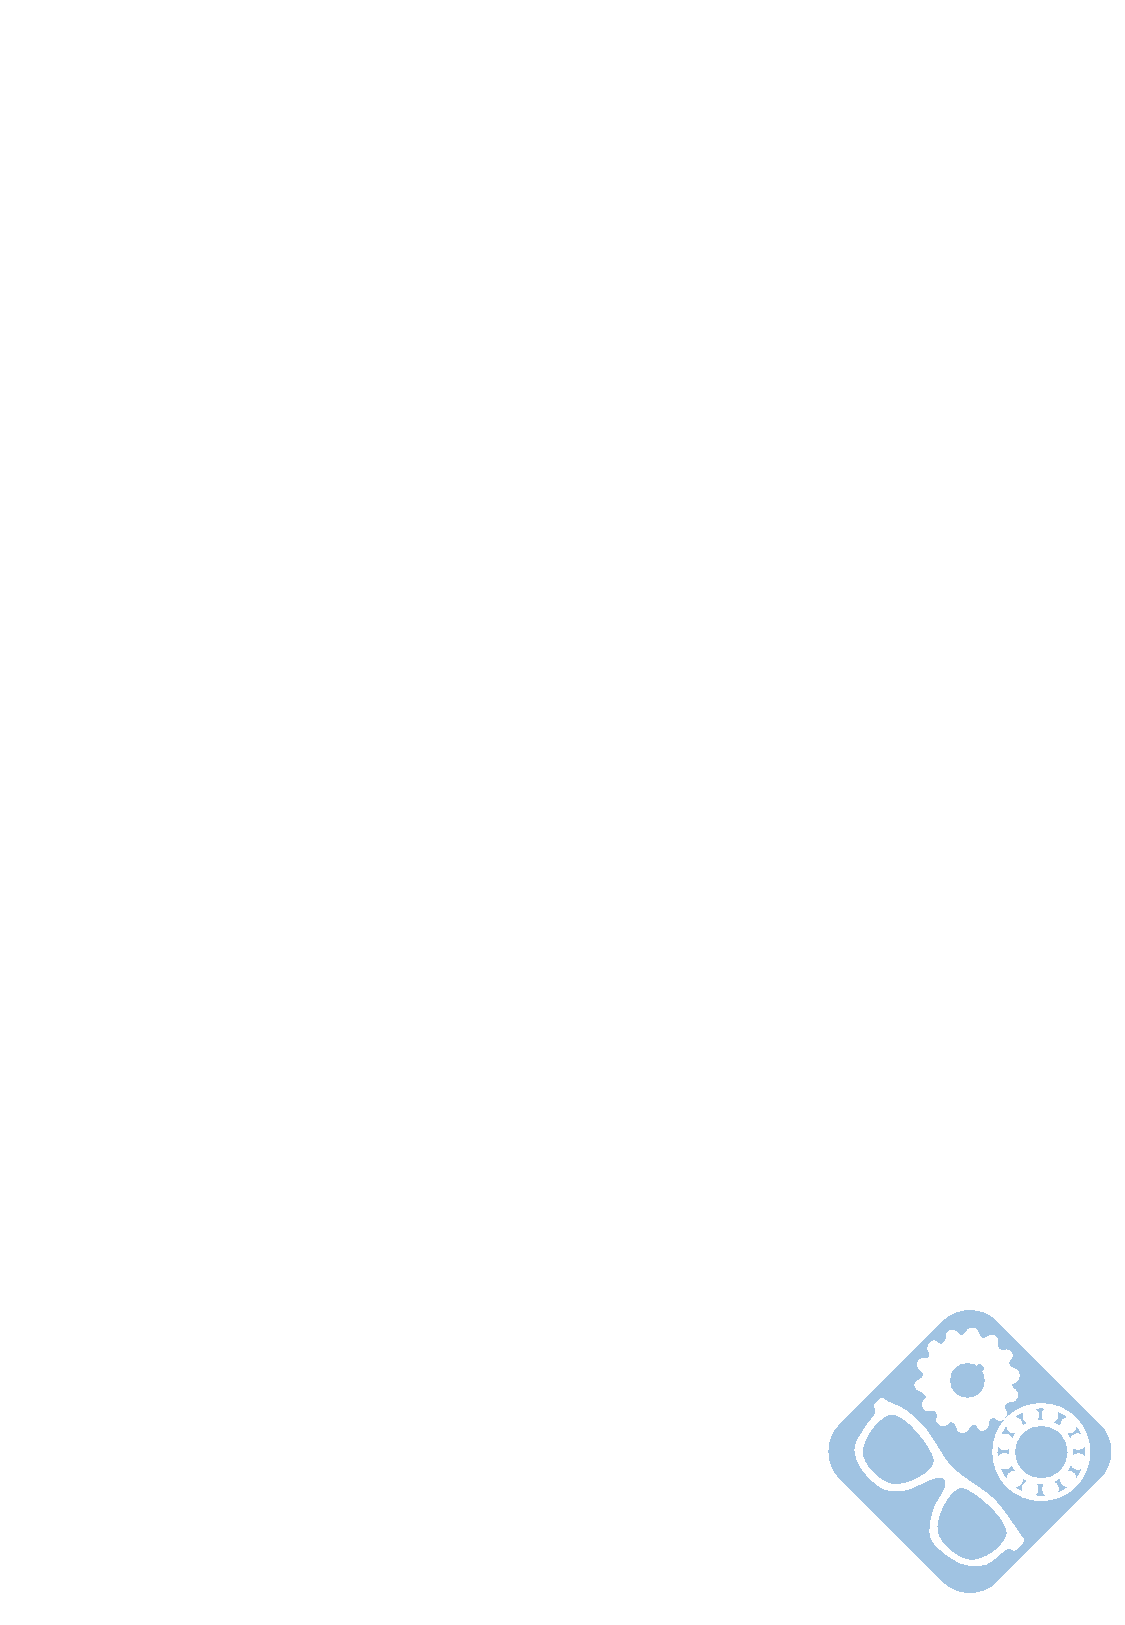
\includegraphics[width=\paperwidth,height=\paperheight,%
keepaspectratio]{../../img/fond4}%
\end{center}
\vfill
}}}

\begin{document}

\AddToShipoutPicture{\BackgroundPicdeux}

\pagestyle{fancy}

\section{Barrière automatique}

\subsection{Le produit barrière automatique et son marché}

\begin{figure}[!h]
 \begin{minipage}{0.3\linewidth}
  \centering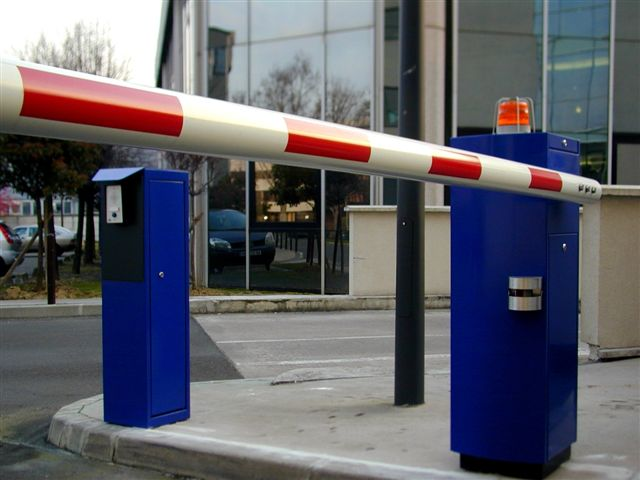
\includegraphics[width=1\linewidth]{img/barriere.jpg}
 \end{minipage}
 \hfill
 \begin{minipage}{0.69\linewidth}
L'évolution croissante du marché automobile mondial, les besoins grandissant de sécurité des biens et personnes font que l'usage de moyens temporaires d'accès conditionnels à des zones accessibles à des véhicules automobiles est des plus répandu.

La solution la plus courante pour répondre à ce besoin est l'utilisation d'une barrière animée d'un mouvement de rotation autour d'un axe horizontal, parallèle à la route.
 \end{minipage}
\end{figure}

\begin{figure}[!h]
  \centering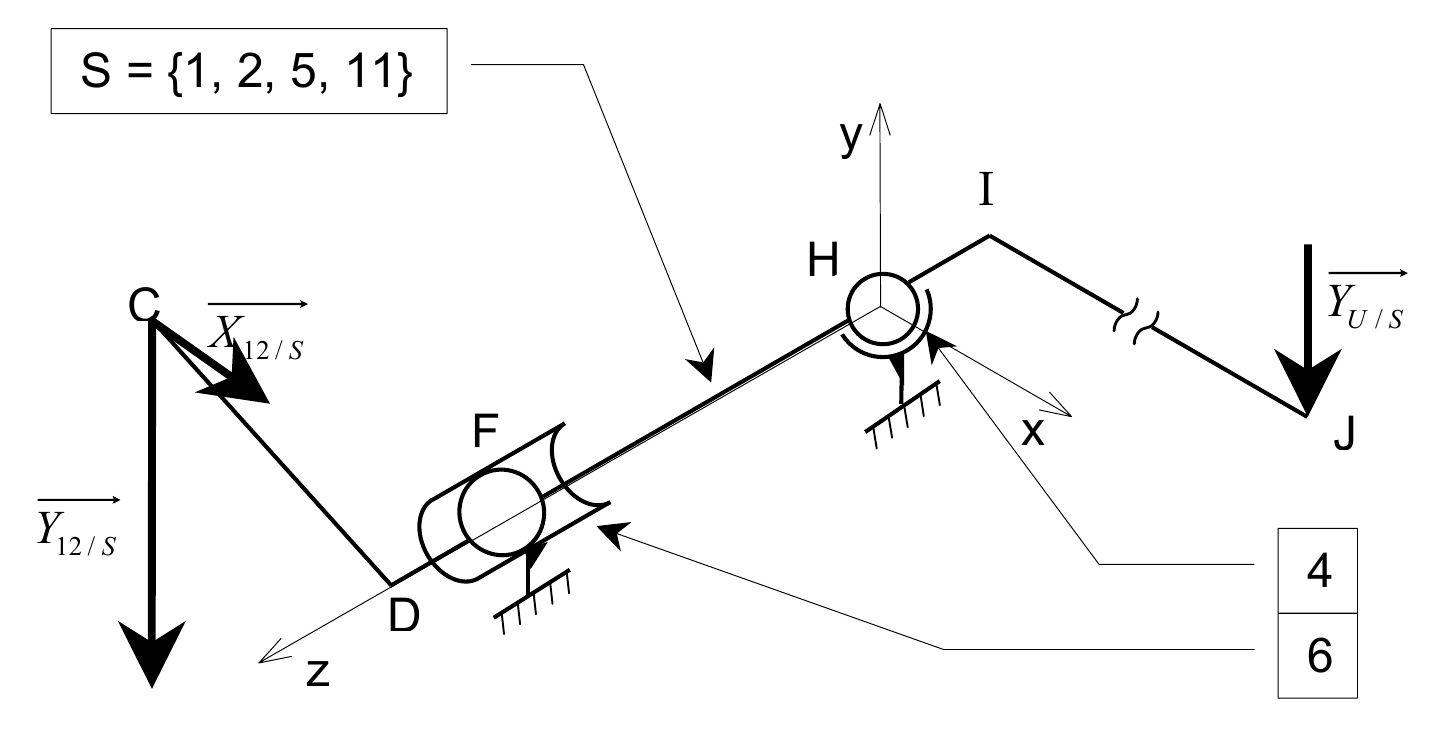
\includegraphics[width=0.7\linewidth]{img/barriere_cin.png}
\end{figure}

$\overrightarrow{DC}=-100\overrightarrow{x}+50 \overrightarrow{y}$, $\overrightarrow{FD}=100.\overrightarrow{z}$, $\overrightarrow{HF}=250.\overrightarrow{z}$, $\overrightarrow{HI}=-100.\overrightarrow{z}$, $\overrightarrow{IJ}=3000.\overrightarrow{x}$.

Action de la tête de bielle 12 sur S au point C :
$\left\{T_{12 \rightarrow S}\right\}=\left\{\begin{array}{c c}
5 & 0 \\
-17.5 & 0 \\
0 & 0
\end{array}\right\}_{C,R}$

Action de l'utilisateur U sur S au point J :
$\left\{T_{U \rightarrow S}\right\}=\left\{\begin{array}{c c}
0 & 0 \\
-0.5 & 0 \\
0 & 0
\end{array}\right\}_{J,R}$

\subsection{Détermination des actions de liaisons}

\textbf{Données :}
Sur la figure est représentée la modélisation de l'ensemble des pièces $S = \left\{1, 2, 5, 11\right\}$ dans la position étudiée, la modélisation de ses guidages, ainsi que les efforts auxquels il est soumis.

\textbf{Hypothèses :}
La position étudiée correspond à une barrière en porte à faux de 3 m, en position horizontale, et à l'extrémité de laquelle un utilisateur U exerce un effort vertical vers le bas de 500 N (selon le cahier des charges).

\begin{itemize}
 \item Toutes les liaisons sont parfaites,
 \item Les actions du ou des ressorts 8 sont négligées,
 \item Les masses des différentes pièces sont négligées,
 \item Les solides sont indéformables.
\end{itemize}

\newpage

\textbf{Notations :}

Les différentes expressions vectorielles seront toujours exprimées dans le repère $R : \left(H,\overrightarrow{x},\overrightarrow{y},\overrightarrow{z}\right)$.

Le torseur des actions mécaniques du solide i sur le solide j, exprimé au point M dans le repère
$\left\{T_{i \rightarrow j}\right\}=\left\{\begin{array}{c c}
X_{i \rightarrow j} & L_{i \rightarrow j} \\
Y_{i \rightarrow j} & M_{i \rightarrow j} \\
Z_{i \rightarrow j} & N_{i \rightarrow j}
\end{array}\right\}_{M,R}$

\paragraph{Question 1:} Donner les expressions particulières des torseurs des actions mécaniques aux points F et H, des paliers 4 et 6, sur S.

\paragraph{Question 2:} Calculer les valeurs des actions mécaniques au point H, de 12 sur S, et de U sur S.

\paragraph{Question 3:} Déterminer les valeurs des actions mécaniques aux points F et H, des paliers 4 et 6, sur S.

\newpage

\section{Manipulateur auto-équilibré}

\subsection{Présentation générale}

\begin{figure}[!h]
 \begin{minipage}{0.3\linewidth}
  \centering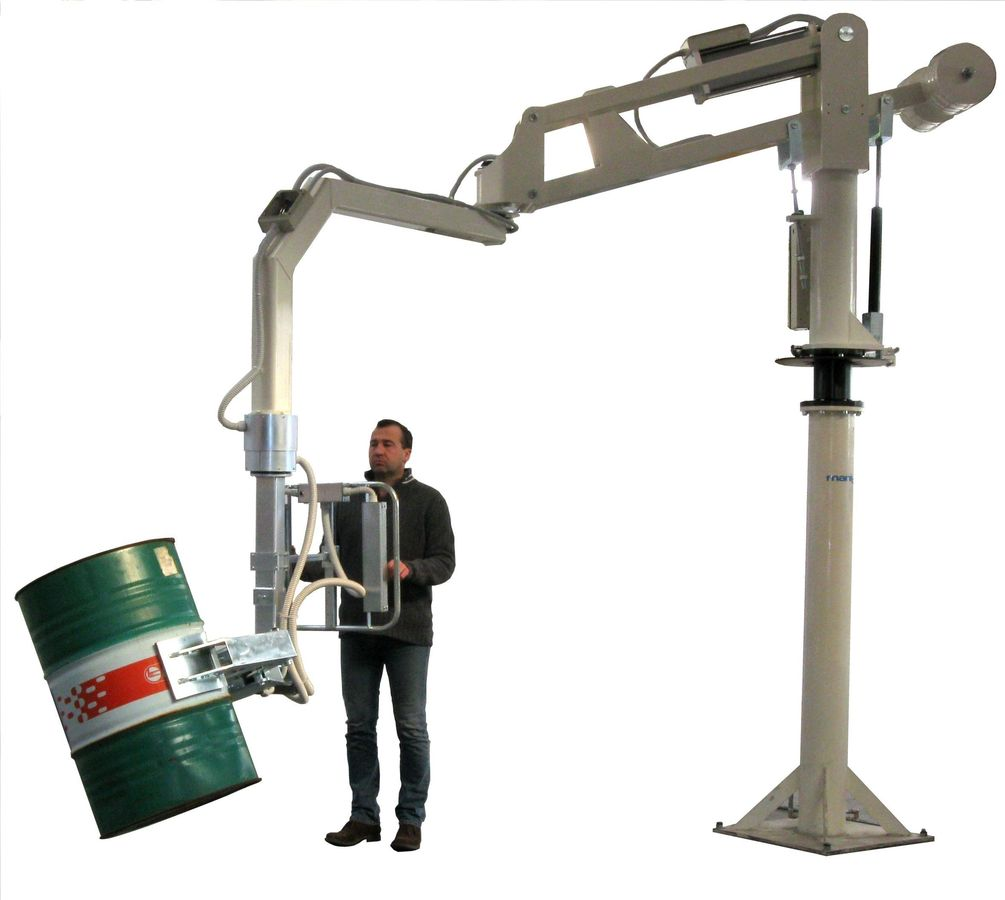
\includegraphics[width=1\linewidth]{img/bras_manipulateur.jpg}
 \end{minipage}
 \hfill
 \begin{minipage}{0.69\linewidth}
Les entreprises industrielles travaillent constamment à l'amélioration de la productivité et de la rentabilité. Sur des opérations de manutention, positionnement, montage, à faible cadence, l'automatisation à outrance et les cellules robotisées ne sont pas rentables...

Les systèmes d'aide à la manutention sont un compromis intéressant.Le sujet a pour thème l'étude du poste de dépose du joint liquide sur le collecteur d'échappement du moteur.

En effet l'employeur maintient une activité humaine (conservation d'emploi) tout en limitant la pénibilité donc en améliorant les conditions de travail, pour des coûts d'investissement modestes.
 \end{minipage}
\end{figure}

\begin{figure}[!h]
  \centering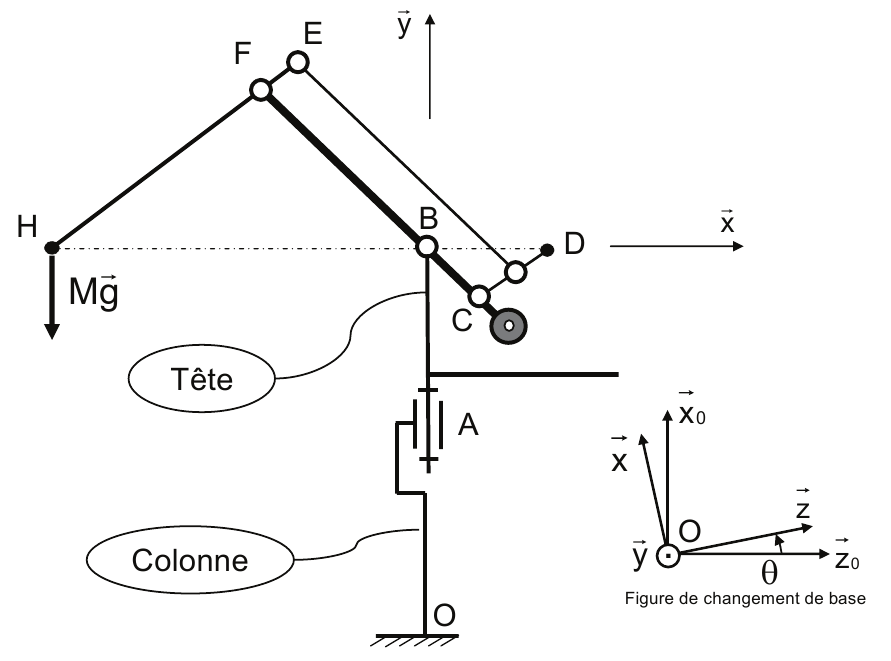
\includegraphics[width=0.6\linewidth]{img/bras_manip_cin.png}
\end{figure}

La tête du bras manipulateur est articulée autour d'un axe vertical par rapport à la colonne fixée au sol. Cette liaison pivot au point A permet à l'utilisateur, lors du déplacement de sa charge, de desservir un volume limité par deux surfaces cylindriques coaxiales.

Pour réaliser cette liaison pivot en limitant l'encombrement et la complexité des pièces adjacentes, le constructeur s'est orienté vers une couronne d'orientation. Les questions qui suivent permettront de choisir cette couronne d'orientation et de définir son implantation.

\textbf{Données :}
\begin{itemize}
 \item $(\overrightarrow{x_0},\overrightarrow{y_0},\overrightarrow{z_0})$ base liée à la colonne donc ici le bâti,
 \item $(\overrightarrow{x},\overrightarrow{y},\overrightarrow{z})$ base liée à la tête du bras.
\end{itemize}

\textbf{Hypothèse :}

Les poids du bras et de la tête sont négligés. Ainsi, les seuls efforts à prendre en compte sont:
\begin{itemize}
 \item le poids de la charge $(\overrightarrow{P}=-M.g.\overrightarrow{y})$,
 \item l'effort dans l'actionneur $(\overrightarrow{Fv}=Fv.\overrightarrow{y}=-k.M.g.\overrightarrow{y})$, en D.
\end{itemize}

\newpage

\paragraph{Question 1:} Exprimer le torseur des actions mécaniques de la tête sur le bras, développées dans la liaison pivot au point B, dans la base $(\overrightarrow{x},\overrightarrow{y},\overrightarrow{z})$ exprimé en B. Calculer les composantes.

\paragraph{Question 2:} Exprimer le torseur des actions mécaniques de la colonne support sur la tête, développées dans la liaison pivot au point A, dans la base $(\overrightarrow{x},\overrightarrow{y},\overrightarrow{z})$ exprimé en A. Calculer les composantes.

\paragraph{Question 2:} Déterminer la valeur de la variable $k$ en fonction des paramètres géométriques du système.

\newpage

\section{Étude géométrique machine de dépose joint liquide}

\subsection{Mise en situation}

La société John Deere conçoit et fabrique du matériel agricole. L'usine, située dans le Loiret, est chargée de la fabrication et du montage des moteurs Diesel de 3, 4, ou 6 cylindres.
Les photos de la figure \ref{fig:image1} montrent la chaîne d'assemblage des moteurs, ceux-ci étant maintenus sur des balancelles.
La pièce qui a pour fonction principale de collecter les gaz d'échappement issus des cylindres pour les envoyer vers le pot d'échappement s'appelle le collecteur d'échappement.
Le sujet a pour thème l'étude du poste de dépose du joint liquide sur le collecteur d'échappement du moteur.

\begin{figure}[htbp]
\begin{center}
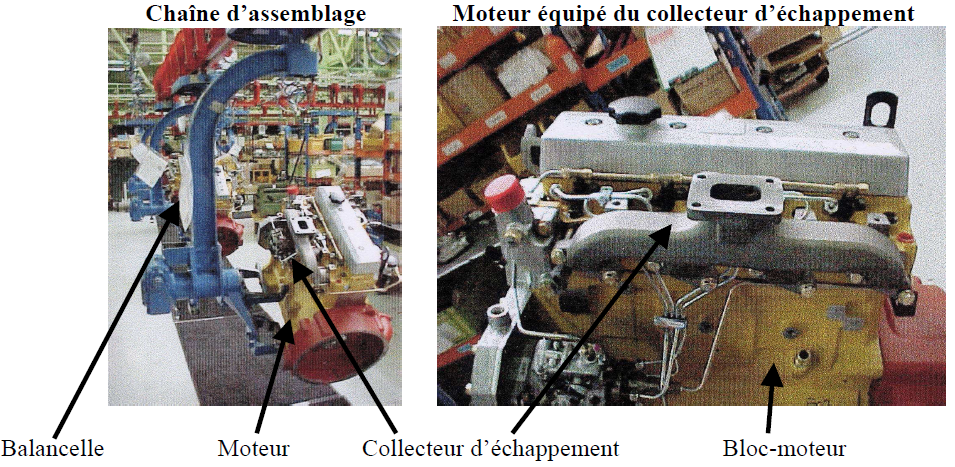
\includegraphics[width=0.6\linewidth]{img/Image2.png}
\caption{Chaîne de fabrication}
\label{fig:image1}
\end{center}
\end{figure}

\subsection{Analyse statique du manipulateur}

L'opérateur utilise le manipulateur pour prendre le collecteur sur le convoyeur.

Il remonte ensuite le collecteur jusqu'à une position où lui-même est debout. Il pourra ainsi plus facilement faire tourner le collecteur pour le placer sur la machine de dépose de joint liquide.

On se place dans cette position stabilisée où le vérin d'équilibrage compense les actions dues au poids du collecteur, juste avant que l'ouvrier ne fasse pivoter le collecteur. Cette position particulière du manipulateur est telle que les bras 2 et 3 soient horizontaux.

\textbf{Hypothèses :} Système simplifié.
\begin{itemize}
 \item Les bras 2 et 3 sont horizontaux. Le vérin 4-6 est vertical.
 \item Les liaisons sont parfaites.
 \item Les poids des différents bras sont négligeables devant celui du collecteur 10.
 \item L'ensemble du manipulateur est en équilibre, et l'opérateur n'agit pas sur le volant de man\oe uvre.
 \item Le collecteur a un centre de gravité placé au point P. On notera $\overrightarrow{P_{10}}$ le poids du collecteur 10. On prendra : $\overrightarrow{g}=10m.s^{-2}$ .
 \item Le problème est plan, dans le plan $(\overrightarrow{x_1},\overrightarrow{y_1})$ de la figure du document 10. Le torseur des actions mécaniques en M d'une pièce i sur une pièce j en projection dans le repère $(\overrightarrow{x_1},\overrightarrow{y_1},\overrightarrow{z_1})$ sera noté $\left\{T_{i \rightarrow j}\right\}=\left\{\begin{array}{c c}
X_{i \rightarrow j} & - \\
Y_{i \rightarrow j} & - \\
- & N_{i \rightarrow j}
\end{array}\right\}_{M,R}$
\end{itemize}

\begin{figure}[htbp]
\begin{center}
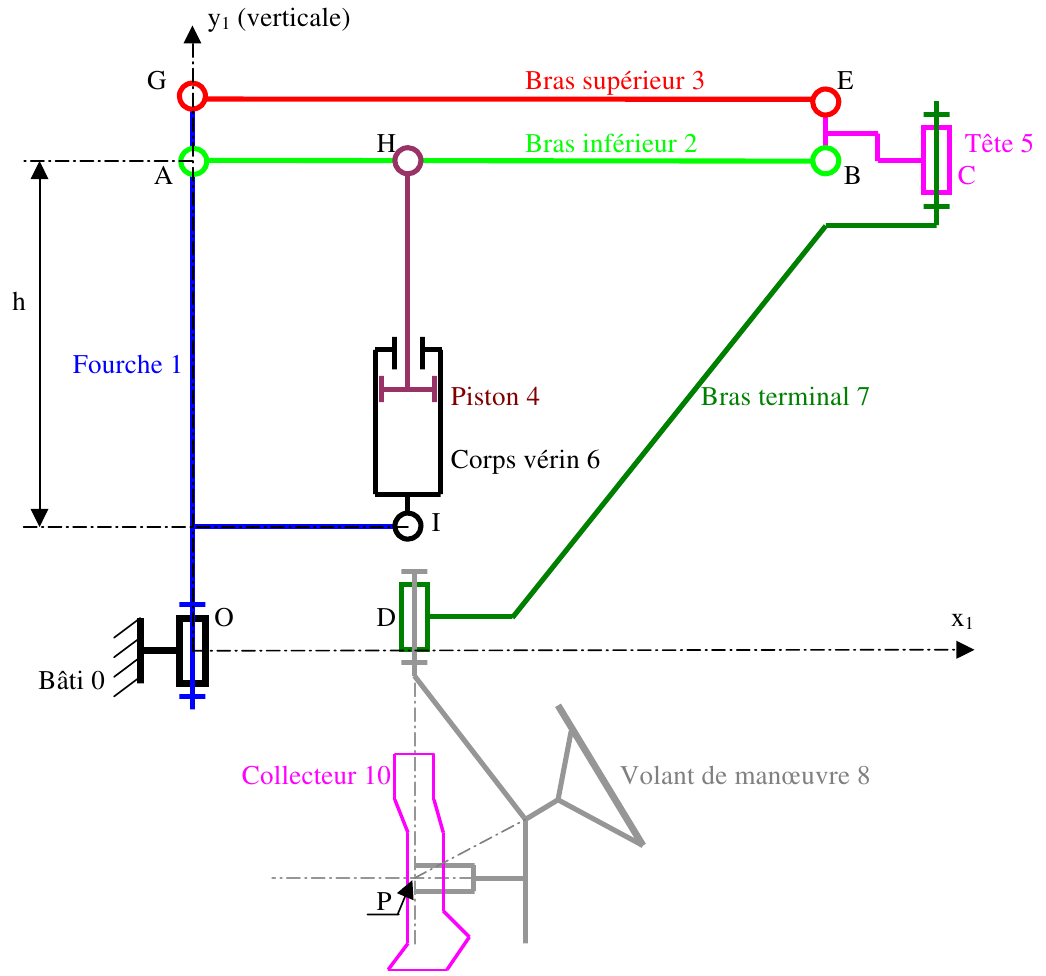
\includegraphics[width=0.6\linewidth]{img/depo_joint_cin.png}
\end{center}
\end{figure}

\paragraph{Question 1:} Isoler le solide $\left\{3\right\}$ et déterminer les 3 équations qui lient les composantes des torseurs statiques.

\paragraph{Question 2:} Isoler les solides $\left\{5,7,8,10\right\}$ et déterminer les 3 équations qui lient les composantes des torseurs statiques.

\paragraph{Question 3:} Isoler les solides $\left\{4,6\right\}$ et déterminer les 3 équations qui lient les composantes des torseurs statiques.

\paragraph{Question 4:} Isoler les solides $\left\{2\right\}$ et déterminer les 3 équations qui lient les composantes des torseurs statiques.

Une étude expérimentale a donné le torseur :

$\left\{A_{1 \rightarrow 2}\right\}=\left\{\begin{array}{c c}
X_{1 \rightarrow 2} & - \\
Y_{1 \rightarrow 2} & - \\
- & 0
\end{array}\right\}_{A,\overrightarrow{x_1},\overrightarrow{y_1},\overrightarrow{z_1}}$

Les relevés donnent : $\overrightarrow{R_{1 \rightarrow 2}}=X_{1 \rightarrow 2}.\overrightarrow{x_1}+Y_{1 \rightarrow 2}.\overrightarrow{y_1}$ avec $X_{1 \rightarrow 2}= -1070 N$ et $Y_{1 \rightarrow 2} = -320 N$

\paragraph{Question 5:} Déterminer par le calcul le torseur des actions de 4 sur 2 au point H noté $\left\{H_{4 \rightarrow 2}\right\}$ en fonction des longueurs a, b et de $Y_{1 \rightarrow 2}$.

\end{document}

\newpage

\section{Funiculaire de Montmartre}

\begin{minipage}{0.4\linewidth}
 \centering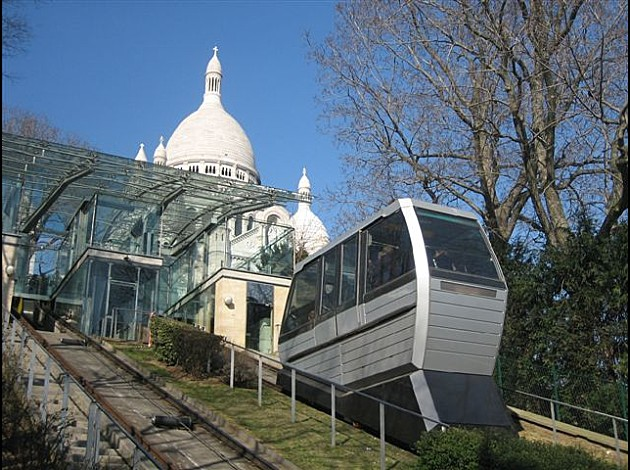
\includegraphics[width=0.7\linewidth]{img/Montmartre.jpg}
\end{minipage}
\hfill
\begin{minipage}{0.57\linewidth}
Un funiculaire est une remontée mécanique équipée de véhicules circulant sur des rails en pente et dont la traction est assurée par un câble.

Il se compose de deux rames reliées par un câble. Le poids du train descendant compense une partie du poids du train montant, cela permet de minimiser l'énergie à fournir par la traction.
\end{minipage}


\end{document}